% Privacy-first section 5: identification without reproduction. The result Erman asked to lead
% the paper. Budget 1.5 pages including Table~\ref{tab:ident} and Figure~\ref{fig:ident}.
% Numbers from outputs/bpe_human/*/scores_*.json, three seeds, verified on one basis; notes 3.59.
\section{A model can identify a person without writing their DNA}
\label{sec:ident}

The safety check this field applies is reproduction: plant a record, ask the model to produce it,
and conclude that a model which produces nothing has retained nothing. This section is the
counterexample. At every checkpoint of every seed we tested, a single-copy human haplotype is
reproduced \emph{exactly zero} times. At those same checkpoints the model names which individual's
haplotype it was trained on, correctly in up to 96\% of cases.

\paragraph{Setup.}
DNABERT-2 fine-tuned on human chromosome~22 with real rare-variant haplotypes as canaries, three
seeds, checkpoints saved along the run. Identification is membership by ranking: the model scores
the planted record against 100 other real rare-variant segments drawn from the same pool, and we
count the cases where the planted one ranks first. Chance is $1/101 = 0.0099$. The segments in the
pool are equally real and equally rare, so the only thing separating a member from a non-member is
whether it was trained on --- which is the comparison a membership claim requires, and a harder one
than ranking against random sequence.

\begin{table}[t]
\centering
\caption{DNABERT-2 on chromosome~22, three seeds, per checkpoint. \emph{id} is identification
(ranked first against 100 real rare segments, chance $0.0099$); \emph{verbatim} is exact recovery of
all 48 target nucleotides. Single-copy verbatim is zero in every cell of this table.}
\label{tab:ident}
\begin{tabular}{lcccc}
\toprule
& & \multicolumn{1}{c}{16 copies} & \multicolumn{2}{c}{1 copy} \\
\cmidrule(lr){3-3}\cmidrule(lr){4-5}
checkpoint & held-out \bits & id & id & verbatim \\
\midrule
round 15 (best held-out) & 1.264 & 0.60 / 0.60 / 0.60 & 0.00 / 0.00 / 0.00 & 0\% \\
round 30                 & 1.296 & 1.00 / 1.00 / 1.00 & 0.00 / 0.00 / 0.00 & 0\% \\
round 50                 & 1.354 & 1.00 / 1.00 / 1.00 & 0.00 / 0.00 / 0.00 & 0\% \\
round 80                 & 1.456 & 1.00 / 1.00 / 1.00 & 0.20 / 0.20 / 0.40 & 0\% \\
round 120                & 1.600 & 1.00 / 1.00 / 1.00 & \textbf{0.80 / 0.70 / 0.80} & 0\% \\
final                    & 1.729 & 1.00 / 1.00 / 1.00 & \textbf{0.94 / 0.92 / 0.96} & 0\% \\
\midrule
never-trained control & --- & \multicolumn{3}{c}{0 of 350 segments, 19 cells} \\
\bottomrule
\end{tabular}
\end{table}

\paragraph{Identification saturates long before reproduction begins.}
Table~\ref{tab:ident} separates the two rulers cleanly. For records planted sixteen times,
identification is already 0.60 at the best held-out checkpoint and reaches 1.00 by round~30, where
verbatim recovery is still 0.10--0.20 and never rises above 0.60 anywhere in the run. For records
planted once, which is the case that matters because one individual's haplotype appears once in a
real cohort, identification climbs from nothing to 0.92--0.96 while verbatim recovery stays at zero
throughout. The two statistics are not the same quantity measured at different sensitivities. They
diverge, and the cheaper one is the one that reads clean. Figure~\ref{fig:ident} shows the two
against each other over the run.

\begin{figure}[t]
\centering
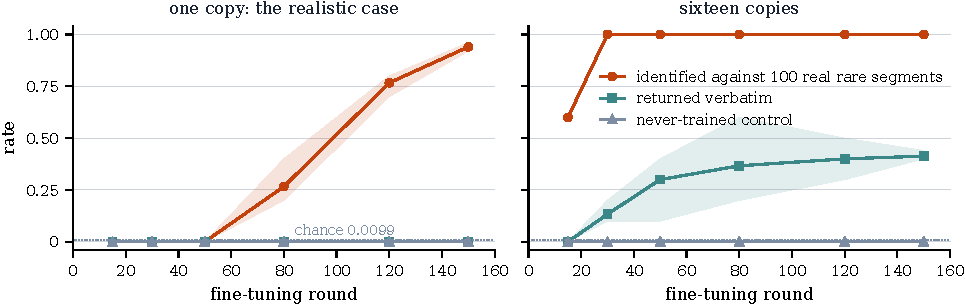
\includegraphics[width=\linewidth]{F6_ident.pdf}
\caption{DNABERT-2 fine-tuned on chromosome~22, three seeds; the band is the range over seeds.
\textbf{Left:} a haplotype planted once, which is the realistic case. Identification rises to 0.94
while verbatim recovery of the same records stays at zero at every checkpoint. \textbf{Right:} the
same records planted sixteen times, where verbatim recovery does move, so the zero on the left is
not a decoder unable to read this family at all. Never-trained controls are flat at zero in both
panels; the dotted line is chance, $0.0099$. Rounds 15--120 use 10 probes per tier and the last
round 50.}
\label{fig:ident}
\end{figure}

The control settles the obvious objection. Across 19 cells and 350 never-trained segments, not one
was ever ranked first. A probe loose enough to manufacture 0.94 out of nothing would have produced
false positives here, and it produced none.

\paragraph{Why this matters more than the reproduction numbers.}
Section~\ref{sec:leak} established that released models return records verbatim at a quality
practitioners would accept, which is the result that is easiest to act on. This one is the result
that is easiest to miss. A team following current practice plants canaries, measures extraction,
reads zero at single copy, and ships. The model they ship will, on being handed a candidate
haplotype, say whether that person was in the cohort: nine times in ten at the end of training, and
better than one in five from round~80 onward, which is well inside the range anyone would train to.
Both numbers therefore have to be reported. Either one on its own gives a misleading account of the
same weights.

\paragraph{A note on what is robust here.}
Identification is a ranking, and rankings are stable under the numerical noise that makes extraction
rates wobble (\S\ref{sec:measure}). Re-scoring a checkpoint months later on the same host after its
floating-point behaviour had changed reproduced every identification rate to the digit --- rank-1 at
$0.800$ before and after, held-out loss identical to four decimals --- while the extraction rate on
the same checkpoint moved by six points. The identification results in this table therefore do not
carry the uncertainty that \S\ref{sec:measure} attaches to the extraction results, and we quote them
without it.
